%\documentclass[iop]{emulateapj}
\documentclass[preprint]{aastex}
%\documentclass[12pt, onecolumn]{emulateapj}
%\documentstyle[aas2pp4,natbib209]{article}

\usepackage{tikz}
\usepackage{natbib}
\usepackage{amsmath}

\usetikzlibrary{shapes.geometric, arrows}
\usetikzlibrary{fit}

\tikzstyle{hyper} = [circle, text centered, draw=black]
\tikzstyle{param} = [circle, text centered, draw=black]
\tikzstyle{data} = [circle, text centered, draw=black, line width=2pt]
\tikzstyle{arrow} = [thick,->,>=stealth]

\newcommand{\myemail}{aimalz@nyu.edu}
\newcommand{\textul}{\underline}

\shorttitle{How to obtain the redshift distribution from probabilistic redshift estimates}
\shortauthors{Malz and Hogg}

\begin{document}

\title{How to obtain the redshift distribution from probabilistic redshift estimates}

\author{Alex Malz\altaffilmark{1} \& David W. Hogg\altaffilmark{1,2,3,4}}
\email{aimalz@nyu.edu}

\altaffiltext{1}{Center for Cosmology and Particle Physics, Department of Physics,
  New York University, 726 Broadway, 9th floor, New York, NY 10003, USA}
\altaffiltext{2}{Simons Center for Computational Astrophysics, 162 Fifth Avenue, 7th floor, New York, NY 10010, USA}
\altaffiltext{3}{Center for Data Science, New York University, 60 Fifth Avenue, 7th floor, New York, NY 10003, USA}
\altaffiltext{4}{Max-Planck-Institut f\"ur Astronomie, K\"onigstuhl 17, D-69117 Heidelberg, Germany}

\begin{abstract}
The redshift distribution $n(z)$ is a crucial ingredient for weak lensing cosmology.  Spectroscopically confirmed redshifts for the dim and numerous galaxies observed by weak lensing surveys are expected to be inaccessible, making photometric redshifts (photo-$z$s) the next best alternative.  Because of the nontrivial inference involved in their determination, photo-$z$ point estimates are being superseded by photo-$z$ probability distribution functions (PDFs).  However, analytic methods for utilizing these new data products in cosmological inference are still evolving.

This paper presents a novel approach to estimating the posterior distribution over $n(z)$ from a survey of galaxy photo-$z$ PDFs based upon a probabilistic graphical model of hierarchical inference.  We present the Cosmological Hierarchical Inference with Probabilistic Photometric Redshifts (CHIPPR) code implementing this technique, as well as its validation on mock data and testing on a subset of BOSS DR10.  CHIPPR yields an accurate characterization of $n(z)$ containing information beyond the best-fit estimator produced by traditional procedures.  The publicly available code is easily extensible to other one-point statistics that depend on redshift.

\end{abstract}

\keywords{catalogs --- cosmology: cosmological parameters --- galaxies: statistics --- gravitational lensing: weak --- methods: analytical --- methods: data analysis --- methods: statistical --- techniques: photometric}

\section{Introduction}
\label{sec:introduction}

The redshift distribution $n(z)$ is necessary for calculating two-point statistics of galaxy properties used to determine the cosmological parameter values that inform our understanding of the evolution of large-scale structure in the universe \citep{masters_mapping_2015}.  Inaccurate estimates of $n(z)$ can significantly impact the constraining power of a galaxy survey, biasing recovery of the cosmological parameters.  For example, if the $n(z)$ used in analysis is offset from the true $n(z)$ by a small, negative constant, it results in underestimating $w_{0}$ and overestimating $\sigma_{8}$ \citep{samuroff_simultaneous_2017}.

Though the redshift density function has traditionally been determined from spectroscopically observed redshifts, modern galaxy surveys including DES, LSST, Euclid, and WFIRST seek to obtain two-point statistics of redshift from samples of galaxies for which spectroscopic redshifts are unavailable, either due to their large numbers or their low brightnesses.  For decades, photometrically estimated redshifts (photo-$z$s) have been the leading alternative to spectroscopically observed redshifts, though they suffer from issues of precision in the form of an intrinsic scatter and accuracy in the form of catastrophic outliers, as well as other systematics imparted by the properties of the survey, data reduction pipeline(s), and assumptions underlying the analysis \citep{baum_photoelectric_1962}.  These weaknesses are illuminated by a probabilistic interpretation of photo-$zs$; if these nontrivial uncertainties were expressed as a probability distribution function (PDF) over redshift, photo-$z$s could be replaced by photo-$z$ PDFs containing more information than a simple point estimate \citep{koo_overview_1999}.  Such data products have been commonly released by photometric galaxy surveys since SDSS DR7 \citep{abazajian_seventh_2009} using a great variety of methods.

Methods for using photo-$z$ PDFs in cosmological inference remain underdeveloped, with many survey pipelines reducing them to familiar point estimators that are compatible with existing technology or engaging with them heuristically in a manner inconsistent with their probabilistic nature.  Stacking photo-$z$ PDFs, or other mathematically equivalent methods, to obtain an estimator of $n(z)$ is especially popular \citep{cunha_estimating_2009, sheldon_photometric_2012}.  However, photo-$z$ PDFs are probabilistic data products that must be handled in a fully consistent, probabilistic manner; hierarchical inference is the only mathematically valid way to do inference with photo-$z$ PDFs and other probabilistic quantities.

It is desirable to create rigorous methods for using photo-$z$ PDFs in inference, beginning with the simplest one-point statistic of redshift, $n(z)$.  In the spirit of \citet{hogg_inferring_2010, foreman-mackey_exoplanet_2014}, this paper derives a mathematically rigorous approach to inferring $n(z)$ in Sec. \ref{sec:method}.  The presentation of a public code implementing this novel technique is given in Sec. \ref{sec:model_specifics}.  The code is validated on mock data and tested on a subset of BOSS DR10 data in Sec. \ref{sec:experiments}.  We conclude and discuss future directions in Sec. \ref{sec:discussion}.

\section{Method}
\label{sec:method}

The redshift distribution $n(z)$ may be understood as the probability of finding a galaxy at a redshift $z$.  We may express $n(z)$ in terms of some functional form $f_{\vec{\theta}}(z)$ with parameters comprising $\vec{\theta}$ according to Eq. \ref{eq:parametrization}.  
\begin{align}
\label{eq:parametrization}
n(z) &\equiv f_{\vec{\theta}}(z)\ \equiv\ p(z|\vec{\theta})
\end{align}
In this work, we wish to characterize the posterior distribution $p(\vec{\theta}|D)$ of the parameters contained in $\vec{\theta}$ defining $n(z)$ given all available data $D$.  The likelihood $p(z|\vec{\theta})$ represents the probability of a random variable, in this case redshift $z$, given the parameters in $\vec{\theta}$ defining the distribution $n(z)$ from which it is drawn.  Our model for inferring $p(\vec{\theta}|D)$ will be introduced in Sec. \ref{sec:derivation}, and alternative methods of estimating $\vec{\theta}$ will be presented in Sec. \ref{sec:alternatives}.

\subsection{Model Specifics}
\label{sec:derivation}

Inference of $p(\vec{\theta}|D)$ is perfectly suited to a hierarchical Bayesian model.  In this problem, the available data $D$ is a catalog of photometry $\{\vec{d}_{i}\}$ of individual galaxies $i$ where each $\vec{d}_{i}$ is a random variable that is a function of its redshift parameter $z_{i}$; the redshift parameters $\{z_{i}\}$ are independently drawn from a function defined by hyperparameters in $\vec{\theta}$.  These physical relationships may be illustrated in Fig. \ref{fig:pgm} by a directed acyclic graph representing a probabilistic graphical model (PGM).
\begin{figure}
\begin{center}
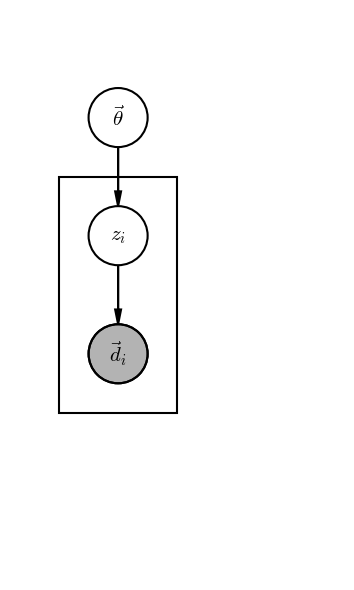
\includegraphics[width=0.5\textwidth]{pgm.png}
\caption{This directed acyclic graph corresponds to a PGM for a hierarchical inference of $p(\vec{\theta}|\{\vec{d}_{i}\})$.  In this graph, all random variables are shown in circles, with observed variables shown in shaded circles.  Relationships between variables are indicated by arrows.  The box indicates that there are a number of copies of the relationships between boxed parameters, each independent of all others.  The hyperparameters $\vec{\theta}$ representing $n(z)$ are at the top.  Independently drawn from a function of the hyperparameters $\vec{\theta}$ are galaxy redshifts $\{z_{i}\}$ below.  The observed galaxy photometry $\{\vec{d}_{i}\}$, shown in shaded circles, is determined by the redshifts above.}
\label{fig:pgm}
\end{center}
\end{figure}
This PGM may be used as the basis for a derivation of the desired hyperposterior $p(\vec{\theta}|\{\vec{d}_{i}\})$, assuming our physical model is complete.  From this point on, we will work solely with log probabilities.

We begin with Eq. \ref{eq:bayes} by applying Bayes' Rule to express the log-hyperposterior $\ln\left[p(\vec{\theta}|\{\vec{d}_{i}\})\right]$ in terms of the log-hyperlikelihood $\ln\left[p(\{\vec{d}_{i}\}|\vec{\theta})\right]$.
\begin{align}
\label{eq:bayes}
\ln\left[p(\vec{\theta}|\{\vec{d}_{i}\})\right] &\propto \ln\left[p(\vec{\theta})\right] + \ln\left[p(\{\vec{d}_{i}\}|\vec{\theta})\right]
\end{align}
To do this, we will choose a log-hyperprior distribution $\ln\left[p(\vec{\theta})\right]$ representing our beliefs about the distribution of the hyperparameters $\vec{\theta}$ in terms of fixed variables that we will assume are known.

The log-hyperlikelihood $\ln\left[p(\{\vec{d}_{i}\}|\vec{\theta})\right]$ contains no explicit reference to redshifts, therefore, we employ the PGM to write the marginalization over the redshifts in Eq. \ref{eq:marginalization}.
\begin{align}
\label{eq:marginalization}
\ln\left[p(\{\vec{d}_{i}\}|\vec{\theta})\right] &= \ln\left[\int\ p(\{\vec{d}_{i}\}|\{z_{i}\})\ p(\{z_{i}\}|\vec{\theta})\ d\{z_{i}\}\right]
\end{align}
We shall handle the two terms in the integral separately.

The first term is the likelihood of all galaxy photometry given all galaxy redshifts.  If we assume independence of galaxy photometry, such that $p(\vec{d}_{i}|\{\vec{d}_{i'\neq i}\}, \{z_{i}\})=p(\vec{d}_{i}|z_{i})$, then we may write Eq. \ref{eq:independence}.
\begin{align}
\label{eq:independence}
\ln\left[p(\{\vec{d}_{i}\}|\{z_{i}\})\right] &= \sum_{i}\ln\left[p(\vec{d}_{i}|z_{i})\right]
\end{align}
The second term may also be expanded by assuming that all galaxy redshifts are drawn independently from $n(z)$.
\begin{align}
\label{eq:poisson}
\ln\left[p(\{z_{i}\}|\vec{\theta})\right] &= \sum_{i}\ln\left[p(z_{i}|\vec{\theta})\right]
\end{align}



Photo-$z$ PDFs, on the other hand, are posteriors, probabilities of a parameter, in this case redshift $z$, given the random variable derived from the parameter, in this case photometric data $\vec{d}$.  Though they are commonly written as $p(z)$, a photo-$z$ PDF for galaxy $i$ in the catalog is truly a posterior $p(z_{i}|\vec{d}_{i})$ where $\vec{d}_{i}$ represents photometric data.

This approach makes several assumptions that must be explicitly stated.
\begin{enumerate}
\item The PGM is an expression of our beliefs about the physics of the problem, and the inference will only be valid to the degree that the model is complete.
\item We must choose a hyperprior $p(\vec{\theta})$; though we aim to choose a sufficiently general hyperprior that will not be a dominant source of information in the hyperposterior, it must still be assumed that whatever hyperprior is chosen will be accurate.
\item We have assumed independence of galaxies in our catalog such that each galaxy's photometry $\vec{d}_{i}$ is independent from all other galaxies' photometry $\{\vec{d}_{i'\neq i}\}$ and all other galaxies' redshifts $\{z_{i'\neq i}\}$.
\end{enumerate}


\section{Alternative methods}
\label{sec:alternatives}

\section{Experiments}
\label{sec:experiments}

\section{Discussion}
\label{sec:discussion}

%\appendix{}

\begin{acknowledgements}
AIM thanks Phil Marshall for advising on the production of usable code, Mohammadjavad Vakili for insightful input on statistics, Geoffrey Ryan for assistance in debugging code, and Boris Leistedt for helpful comments provided in the preparation of this paper.
\end{acknowledgements}

\bibliographystyle{apj}
\bibliography{references}

\end{document}